%!TEX root = ../username.tex
\chapter{Genetic Algorithms} \label{ga}

In this project, the melodies generated by the Markov model are used as the initial population for the genetic algorithm.

\section{Fitness Function} \label{ga:fitness}

In several previous papers, the authors discuss the use of interactive fitness functions \cite{papadopoulos_ai_1999, mcvicar_autoguitartab:_2015}.
With this method, a human listens to the melodies and selects the best from each generation to be used as the parents of the next generation.
This method does well at picking the most pleasing music to human ears, but it requires humans to listen to the music, which is slow and can lead to fatigue on the part of the evaluators.

Rather than rely on humans who may become tired, or may vary their definition of good music over time, we want to use an automated fitness function.
Music from the common practice period of Western music, which lasted from the late Baroque period through the Romantic period (1650-1900), generally followed a complex set of rules regarding harmony, rhythm, and duration.
We could manually define a function that applies some penalty for breaking a rule, but this approach could be highly error prone and require lots of manual tweaking.

Rather, it is often good enough to approximate a fitness function using what we call a \textit{surrogate model}. % cite a paper on this
Some authors discuss techniques for fitness functions as applied to music \cite{papadopoulos_ai_1999, de_freitas_originality_2011, alfonseca_fitness_2006}.
For example, Alan de Freitas and Frederico Guimaraes use a fitness function that penalizes any note outside of the C Major scale, while George Papadopoulos and Geraint Wiggins use a fitness function that considers several characteristics of the melody, including consecutive intervals, note durations, and contour.
% TODO write about accuracy results from these authors
In this project we use an artificial neural network as the surrogate model.
We expect the neural network to pick up on which rules are the most important, altering its weights accordingly.
Because music has temporal properties, the type of neural network used in this project is a \textit{long short-term memory} (LSTM) network.
An LSTM network is a special type of \textit{recurrent neural network}, where nodes link back to themselves. % TODO write about LSTM networks here

The classification we use is binary: is the chunk of music run through the network similar to the chunks of music used to train the network?
We expect the network might pick up on attributes such as how long a note lasts, what the pitch of a note is, and its relation to the notes around it.
However, we cannot know for certain that the network decides is important before training.

In our corpus of music, the sixteenth note is most commonly the smallest rhythmic value in a piece of music, so we first preprocess the music data by converting all rhythms to consecutive sixteenth notes.
The motivation for this method, rather than trying to encode the rhythm in another way comes from Peter Todd \cite{todd_connectionist_1989}.
We perform additional preprocessing by \textit{one-hot encoding} the pitch of each note.
To limit the range of octaves that can appear in our music, we use the MIDI values for each pitch.
Because standard MIDI values range from $0$ to $127$, we can one-hot encode the pitch as an array of zeros with a $1$ at the index of the MIDI number we want to represent.

Unlike a traditional neural network, an input sample is not entered all at once.
Instead, each note enters the network one at a time.
For this project, we consider four measures of music as input to the neural network.
With our rhythmic encoding of sixteenth notes, this means for each music sample we input $16 * 4 = 64$ notes to the network.
In more general terminology, each note is a \textit{chunk}.
Since each note consists of a single one-hot encoded pitch, the \textit{chunk size} is $128$.
Somewhat arbitrarily, we pass each input through $128$ neurons in the network.
The output of the network is a an array containing two value, which are the network's certainty that the input is or is not a good melody.

During training, in addition to samples of correct music from our corpus, we also feed the network samples of random noise as incorrect examples.

Using this network setup, we were able to achieve up to $99\%$ accuracy during training.

\section{Mutations} \label{ga:mutate}

There are several natural mutations to consider when working with music.
Two common compositional techniques are inversion and retrograde.
Inversion takes a section of music, generally a couple of measures, and inverts all the intervals, so an interval up becomes the same interval down.
Retrograde reverses the order of one or both of the rhythms and pitches of a section of music.
Retrograde and inverse can also be combined, to yield retrograde-inverse.
Typically, the section is inverted, and the new notes are then read backwards, though some composers, such as Igor Stravinsky, reversed the order of the notes first.
See Figure \ref{fig:p-r-i-ri} for an example of inversion, retrograde, and retrograde-inversion.
These techniques are especially common in twelve tone music, which was developed during the early twentieth century by Arnold Schoenberg, though they can also be found in other types of music. % TODO give examples
In our genetic algorithm, we apply these compositional techniques to the melodies from the previous generation to produce new candidates for the current generation.

\begin{figure}
	\centering
	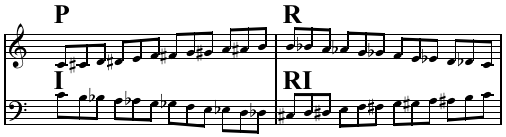
\includegraphics[width=\linewidth]{figures/P-R-I-RI.png} % TODO cite image https://commons.wikimedia.org/wiki/File:P-R-I-RI.png
	\caption{Common  clockwise from the top left: prime (original form), retrograde, inverse, and retrograde-inverse.}
	\label{fig:p-r-i-ri}
\end{figure}

A big idea when working with genetic algorithms is \textit{crossover}, where members of the population are spliced together to create new candidates.
Finally, to maintain diversity in the population, we introduce some random changes to the population at a rate determined by some volatility factor, which can either stay constant or change over time.

\section{Manipulating Melodies} \label{ga:manip}


